\begin{pastexam}[label={px:ntust-107-ice-06}]{臺科大資工所 107 學年度 第 6 題}
（問答）

Given an ordered number sequence as follows: 50, 83, 10, 19, 5, 78, 39, 99, 77, 18, 1, 8.
Please answer the following questions. (40\%)
\begin{enumerate}[label=(\alph*)]
\item Please construct a binary search tree by referring to the number sequence. (5\%)
\item Based on the binary search tree you constructed, please traverse the tree using post-order
scan. (5\%)
\item Based on the post-order sequence, please sort the numbers by insertion sort and merge sort,
respectively (you should write down all the steps). (10\%)
\item After we sequentially delete nodes 1, 77, and 83, please draw down all of the possible
binary search trees and then write down their in-order traversal sequences. (20\%)
\end{enumerate}
\end{pastexam}

\begin{pastsoln}
\textbf{(a)} 照順序從空樹一個一個插入（資結書虛擬碼~9.6）：每個數從根往下比，比目前節點小往左、
大往右，走到空位就接上去。
\begin{itemize}
\item $50$ 當根。 $83 > 50$，接在 $50$ 右邊。 $10 < 50$，接在 $50$ 左邊。
\item $19$：$< 50$ 往左，$> 10$ 往右，接在 $10$ 右邊。 $5$：$< 50$、$< 10$，接在 $10$ 左邊。
\item $78$：$> 50$、$< 83$，接在 $83$ 左邊。 $39$：$< 50$、$> 10$、$> 19$，接在 $19$ 右邊。
\item $99$：$> 50$、$> 83$，接在 $83$ 右邊。 $77$：$> 50$、$< 83$、$< 78$，接在 $78$ 左邊。
\item $18$：$< 50$、$> 10$、$< 19$，接在 $19$ 左邊。 $1$：$< 50$、$< 10$、$< 5$，接在 $5$ 左邊。
$8$：$< 50$、$< 10$、$> 5$，接在 $5$ 右邊。
\end{itemize}
\begin{center}
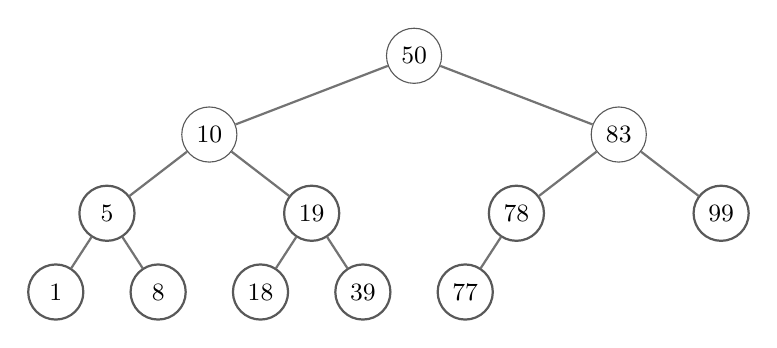
\begin{tikzpicture}[level distance=10mm,
  every node/.style={circle,draw=black!65,minimum size=7mm,inner sep=0pt,font=\small},
  edge from parent/.style={draw=black!55,thick},
  level 1/.style={sibling distance=52mm},
  level 2/.style={sibling distance=26mm},
  level 3/.style={sibling distance=13mm}]
\node {50}
  child {node {10}
    child {node {5}
      child {node {1}}
      child {node {8}}}
    child {node {19}
      child {node {18}}
      child {node {39}}}}
  child {node {83}
    child {node {78}
      child {node {77}}
      child[missing]}
    child {node {99}}};
\end{tikzpicture}
\end{center}

\textbf{(b)} 後序是「左子樹、右子樹、根」（資結書第~7.3~節）。 左子樹 $10$ 的後序是
$1, 8, 5$（$5$ 的子樹）、$18, 39, 19$（$19$ 的子樹）、$10$；右子樹 $83$ 的後序是
$77, 78$、$99$、$83$；最後是根 $50$：
\[
1,\ 8,\ 5,\ 18,\ 39,\ 19,\ 10,\ 77,\ 78,\ 99,\ 83,\ 50.
\]

\textbf{(c)} 都排成由小到大，輸入是 (b) 的後序序列。

\textbf{插入排序}（資結書第~1.3~節、虛擬碼~1.3）：第 $j$ 輪把第 $j$ 個數插進前面已排好的那一段，
比它大的往右挪一格。 下表每一列是那一輪做完的陣列，直線 $\mid$ 左邊是已排好的部分。
\begin{center}
\small
\begin{tabular}{ccll}
\toprule
輪 & 插入 & 這一輪之後的陣列 & 往右挪的數 \\
\midrule
開始 & & $1 \mid 8, 5, 18, 39, 19, 10, 77, 78, 99, 83, 50$ &  \\
1 & $8$ & $1, 8 \mid 5, 18, 39, 19, 10, 77, 78, 99, 83, 50$ & — \\
2 & $5$ & $1, \mathbf{5}, 8 \mid 18, 39, 19, 10, 77, 78, 99, 83, 50$ & $8$ \\
3 & $18$ & $1, 5, 8, 18 \mid 39, 19, 10, 77, 78, 99, 83, 50$ & — \\
4 & $39$ & $1, 5, 8, 18, 39 \mid 19, 10, 77, 78, 99, 83, 50$ & — \\
5 & $19$ & $1, 5, 8, 18, \mathbf{19}, 39 \mid 10, 77, 78, 99, 83, 50$ & $39$ \\
6 & $10$ & $1, 5, 8, \mathbf{10}, 18, 19, 39 \mid 77, 78, 99, 83, 50$ & $39, 19, 18$ \\
7 & $77$ & $1, 5, 8, 10, 18, 19, 39, 77 \mid 78, 99, 83, 50$ & — \\
8 & $78$ & $1, 5, 8, 10, 18, 19, 39, 77, 78 \mid 99, 83, 50$ & — \\
9 & $99$ & $1, 5, 8, 10, 18, 19, 39, 77, 78, 99 \mid 83, 50$ & — \\
10 & $83$ & $1, 5, 8, 10, 18, 19, 39, 77, 78, \mathbf{83}, 99 \mid 50$ & $99$ \\
11 & $50$ & $1, 5, 8, 10, 18, 19, 39, \mathbf{50}, 77, 78, 83, 99$ & $99, 83, 78, 77$ \\
\bottomrule
\end{tabular}
\end{center}
粗體是這一輪插入的數。 這個序列已經「大致排好」，挪動只有 $1 + 1 + 3 + 1 + 4 = 10$ 次，
等於序列裡的逆序對個數。

\textbf{合併排序}（資結書虛擬碼~14.5，由上而下）：每次從中間切開，$q = \lfloor (p + r)/2
\rfloor$，奇數個時左半邊多一個；兩半各自遞迴排好後合併（虛擬碼~14.4）。 切開的過程：
\[
\begin{aligned}
&[1, 8, 5, 18, 39, 19 \mid 10, 77, 78, 99, 83, 50] \\
&[1, 8, 5 \mid 18, 39, 19] \quad [10, 77, 78 \mid 99, 83, 50] \\
&[1, 8 \mid 5]\ \ [18, 39 \mid 19] \quad [10, 77 \mid 78]\ \ [99, 83 \mid 50] \\
&[1 \mid 8]\quad\ \ [18 \mid 39] \qquad\quad\ \ [10 \mid 77] \qquad\ \ [99 \mid 83]
\end{aligned}
\]
接著由下往上合併，照遞迴實際做的順序：
\begin{center}
\small
\begin{tabular}{cll}
\toprule
步 & 合併 & 結果 \\
\midrule
1 & $[1]$ 和 $[8]$ & $[1, 8]$ \\
2 & $[1, 8]$ 和 $[5]$ & $[1, 5, 8]$ \\
3 & $[18]$ 和 $[39]$ & $[18, 39]$ \\
4 & $[18, 39]$ 和 $[19]$ & $[18, 19, 39]$ \\
5 & $[1, 5, 8]$ 和 $[18, 19, 39]$ & $[1, 5, 8, 18, 19, 39]$ \\
6 & $[10]$ 和 $[77]$ & $[10, 77]$ \\
7 & $[10, 77]$ 和 $[78]$ & $[10, 77, 78]$ \\
8 & $[99]$ 和 $[83]$ & $[83, 99]$ \\
9 & $[83, 99]$ 和 $[50]$ & $[50, 83, 99]$ \\
10 & $[10, 77, 78]$ 和 $[50, 83, 99]$ & $[10, 50, 77, 78, 83, 99]$ \\
11 & $[1, 5, 8, 18, 19, 39]$ 和 $[10, 50, 77, 78, 83, 99]$ & $[1, 5, 8, 10, 18, 19, 39, 50, 77, 78, 83, 99]$ \\
\bottomrule
\end{tabular}
\end{center}
兩種方法的結果都是 $1, 5, 8, 10, 18, 19, 39, 50, 77, 78, 83, 99$。 題目沒有指定合併排序的切法，
用由下而上的版本（資結書虛擬碼~14.6，先兩兩合併成長度 $2$，再合成長度 $4$、$8$，最後 $8$ 和
$4$ 合成 $12$）也可以，寫清楚用哪一種、每一步的結果就好。

\textbf{(d)} 依序在 (a) 的樹上刪除（資結書第~9.2~節）。
\begin{itemize}
\item 刪除 $1$：葉節點，直接拿掉，$5$ 只剩右子節點 $8$。
\item 刪除 $77$：葉節點，直接拿掉，$78$ 變成葉節點。
\item 刪除 $83$：有兩個子節點（$78$ 和 $99$）。 要找一個節點取代它，有兩種做法，結果不同：
用\textbf{前驅}（左子樹的最大值 $78$）取代，或用\textbf{後繼}（右子樹的最小值 $99$）取代。
\end{itemize}
前兩次刪除只有一種結果，所以「所有可能的樹」就是第三步的這兩棵：
\begin{center}
\begin{minipage}{0.48\linewidth}\centering
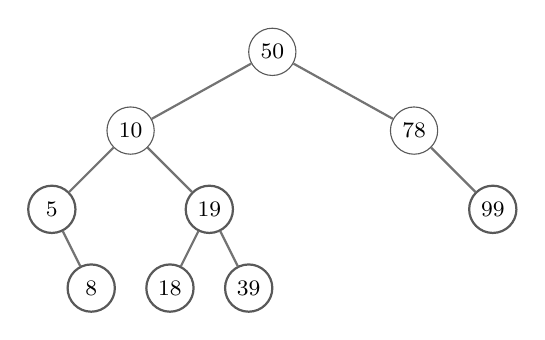
\begin{tikzpicture}[level distance=10mm,
  every node/.style={circle,draw=black!65,minimum size=6mm,inner sep=0pt,font=\footnotesize},
  edge from parent/.style={draw=black!55,thick},
  level 1/.style={sibling distance=36mm},
  level 2/.style={sibling distance=20mm},
  level 3/.style={sibling distance=10mm}]
\node {50}
  child {node {10}
    child {node {5}
      child[missing]
      child {node {8}}}
    child {node {19}
      child {node {18}}
      child {node {39}}}}
  child {node {78}
    child[missing]
    child {node {99}}};
\end{tikzpicture}

{\footnotesize (1) 用前驅 $78$ 取代 $83$}
\end{minipage}\hfill
\begin{minipage}{0.48\linewidth}\centering
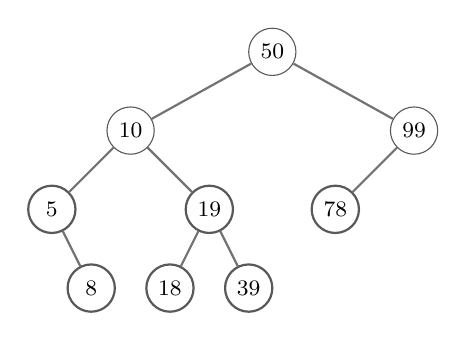
\begin{tikzpicture}[level distance=10mm,
  every node/.style={circle,draw=black!65,minimum size=6mm,inner sep=0pt,font=\footnotesize},
  edge from parent/.style={draw=black!55,thick},
  level 1/.style={sibling distance=36mm},
  level 2/.style={sibling distance=20mm},
  level 3/.style={sibling distance=10mm}]
\node {50}
  child {node {10}
    child {node {5}
      child[missing]
      child {node {8}}}
    child {node {19}
      child {node {18}}
      child {node {39}}}}
  child {node {99}
    child {node {78}}
    child[missing]};
\end{tikzpicture}

{\footnotesize (2) 用後繼 $99$ 取代 $83$}
\end{minipage}
\end{center}
樹 (1)：$78$ 是 $83$ 左子樹的最大值，它沒有右子節點（刪掉 $77$ 後它是葉節點），搬到 $83$ 的位置，
$99$ 留在右邊。 樹 (2)：$99$ 是 $83$ 右子樹的最小值，它沒有左子節點，搬上去之後 $78$ 是它的左子節點。

兩棵樹的中序走訪相同，都是
\[
5,\ 8,\ 10,\ 18,\ 19,\ 39,\ 50,\ 78,\ 99.
\]
這不是巧合：二元搜尋樹的中序走訪一定是鍵值由小到大，刪除只是拿掉一個鍵值，不管用前驅還是後繼，
剩下的九個數排好就是這個順序。 兩棵樹的差別要看前序或後序才看得出來，例如前序分別是
$50, 10, 5, 8, 19, 18, 39, 78, 99$ 和 $50, 10, 5, 8, 19, 18, 39, 99, 78$。
\end{pastsoln}
